% !TeX program = xelatex
\documentclass[a4paper,10pt]{article}

% ============================================================================
% កញ្ចប់បណ្ណាល័យ (Packages) – តាមលំនាំស្តង់ដារ អនុវិទ្យាល័យព្រះក្រសាំង (ls_plan.tex)
% បរិបទ៖ ថ្នាក់រៀនគ្មានស្លាយ LCD – បង្រៀនដោយប្រើក្ដារខៀន សៀវភៅគោល និងសន្លឹកកិច្ចការស-ខ្មៅ
% ============================================================================
\usepackage[a4paper, left=0.95cm, right=0.95cm, top=0.85cm, bottom=0.92cm, footskip=0.52cm]{geometry}
\usepackage{amsmath, amssymb}
\usepackage{unicode-math}
\usepackage{fontspec}
\usepackage{array, longtable, multirow, colortbl}
\usepackage[table]{xcolor}
\usepackage{enumitem}
\usepackage{pifont}
\usepackage{fancyhdr}
\usepackage{tikz}
\usetikzlibrary{calc, arrows.meta, positioning, babel}

\makeatletter
\let\@expl@@@mark@update@singlecol@structures@@\relax
\makeatother

\providecommand{\NGSFindFonts}{%
  \IfFileExists{C:/Windows/Fonts/cambria.ttc}{%
    \def\NGSSysPath{C:/Windows/Fonts/}%
    \def\NGSUserPath{C:/Users/KIT/AppData/Local/Microsoft/Windows/Fonts/}%
  }{%
    \IfFileExists{./fonts/KhmerOSsiemreap.ttf}{\def\NGSSysPath{./fonts/}\def\NGSUserPath{./fonts/}}{%
    \IfFileExists{../fonts/KhmerOSsiemreap.ttf}{\def\NGSSysPath{../fonts/}\def\NGSUserPath{../fonts/}}{%
    \IfFileExists{../../fonts/KhmerOSsiemreap.ttf}{\def\NGSSysPath{../../fonts/}\def\NGSUserPath{../../fonts/}}{%
    \IfFileExists{../../../fonts/KhmerOSsiemreap.ttf}{\def\NGSSysPath{../../../fonts/}\def\NGSUserPath{../../../fonts/}}{%
    \IfFileExists{../../../../fonts/KhmerOSsiemreap.ttf}{\def\NGSSysPath{../../../../fonts/}\def\NGSUserPath{../../../../fonts/}}{%
    \IfFileExists{../../../../../fonts/KhmerOSsiemreap.ttf}{\def\NGSSysPath{../../../../../fonts/}\def\NGSUserPath{../../../../../fonts/}}{%
    \IfFileExists{../../../../../../fonts/KhmerOSsiemreap.ttf}{\def\NGSSysPath{../../../../../../fonts/}\def\NGSUserPath{../../../../../../fonts/}}{%
      \def\NGSSysPath{../../../../../../../fonts/}\def\NGSUserPath{../../../../../../../fonts/}%
    }}}}}}}%
  }%
}
\NGSFindFonts

\setmathfont[Path={\NGSSysPath}, FontIndex=1, Scale=1.02]{cambria.ttc}
\defaultfontfeatures{Ligatures=TeX}

\setmainfont[
  Path={\NGSUserPath},
  Extension=.ttf,
  Script=Khmer,
  BoldFont={KhmerOSsiemreap},
  BoldFeatures={FakeBold=1.8},
  ItalicFont={KhmerOSsiemreap},
  ItalicFeatures={FakeSlant=0.25},
  BoldItalicFont={KhmerOSsiemreap},
  BoldItalicFeatures={FakeBold=1.8, FakeSlant=0.25}
]{KhmerOSsiemreap}

\newfontfamily\muol[Path={\NGSUserPath}, Extension=.ttf, Script=Khmer]{KhmerOSmuollight}
\newfontfamily\TimesEn[Path={\NGSSysPath}, Extension=.ttf, BoldFont={timesbd}, ItalicFont={timesi}, BoldItalicFont={timesbi}]{times}
\newfontfamily\NagaBold[Path={\NGSUserPath}, Extension=.ttf]{AKbalthom Naga Bold}
\newfontfamily\CalibriFont[Path={\NGSSysPath}, Extension=.ttf]{calibri}
\newfontfamily\Tacteing[Path={\NGSUserPath}]{TACTENG.TTF}
\newfontfamily\CourierBullet[Path={\NGSSysPath}, Extension=.ttf]{cour}
\newcommand{\wcirc}{{\CourierBullet\fontsize{9.5pt}{11pt}\selectfont o}}

\XeTeXlinebreaklocale "km"
\XeTeXlinebreakskip = 0pt plus 1pt minus 0.1pt

\definecolor{stepgray}{HTML}{D9D9D9}
\definecolor{headgray}{HTML}{F2F2F2}
\definecolor{boxgray}{HTML}{D9D9D9}
\definecolor{darkred}{HTML}{C00000}
\definecolor{red5e}{HTML}{FF0000}

\pagestyle{fancy}
\fancyhf{}
\renewcommand{\headrulewidth}{0pt}
\fancyfoot[R]{\CalibriFont\fontsize{11pt}{13pt}\selectfont\thepage}

\setlength{\parindent}{0pt}
\setlength{\parskip}{0pt}
\setlength{\tabcolsep}{3.8pt}

\newcolumntype{L}[1]{>{\raggedright\arraybackslash}p{#1}}

\newcommand{\en}[1]{{\TimesEn #1}}
\newcommand{\enbf}[1]{{\TimesEn\textbf{#1}}}
\newcommand{\unit}[1]{\,\text{\en{#1}}}
\newcommand{\fiveE}[1]{{\NagaBold\fontsize{9.5pt}{13pt}\selectfont\textcolor{red5e}{#1}}}
\newcommand{\timenote}[1]{\textcolor{darkred}{\textit{#1}}}
\newcommand{\graybox}[1]{\colorbox{boxgray}{\strut\hspace{2pt}#1\hspace{2pt}}}
\newcommand{\ditem}{\tikz[baseline=-0.5ex]\fill (0,0.42ex) -- (0.42ex,0) -- (0,-0.42ex) -- (-0.42ex,0) -- cycle;\hspace{0.3em}}
\newcommand{\cnum}[1]{{\fontsize{10.5pt}{12pt}\selectfont\ding{\numexpr171+#1\relax}}\hspace{0.2em}}
\newcommand{\cfig}[1]{\par\vspace{4pt}{\centering #1\par}\vspace{4pt}}
\newcommand{\stepheader}[1]{\multicolumn{3}{|c|}{\cellcolor{stepgray}\muol #1} \\* \noalign{\hrule height 0.4pt}}
\newcommand{\khmflourish}{{\Tacteing\fontsize{36pt}{14pt}\selectfont\raisebox{-5pt}{3}}}

% ============================================================================
% ម៉ាក្រូរូបភាពគរុកោសល្យស-ខ្មៅ (Proportional B&W TikZ Diagrams)
% ============================================================================

% ១. E1 Engage: ប្រៀបធៀបត្រីធាការេទ្វេធា x^2-2x+1 ទល់នឹង ត្រីធាទូទៅ x^2-2x-8 (ទំ.៧១)
\newcommand{\figEngageALGEight}{%
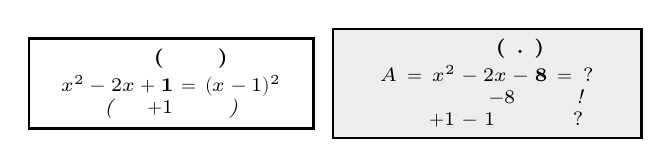
\begin{tikzpicture}[every node/.style={font=\scriptsize, text=black}, >=Stealth]
  \node[draw=black, line width=0.9pt, fill=white, text width=3.35cm, align=center, inner sep=3.8pt] (known) at (0,0) {
    \textbf{ម៉ោងមុន (ការេទ្វេធា)៖}\\[2pt]
    $x^2 - 2x + \mathbf{1} = (x-1)^2$\\
    \textit{(តួចុង $+1$ ជាការេពិត)}
  };
  \node[draw=black, line width=0.9pt, fill=gray!14, text width=3.65cm, align=center, inner sep=3.8pt, right=6pt of known] (newt) {
    \textbf{បញ្ហាថ្ងៃនេះ (ទំ.៧១)៖}\\[2pt]
    $A = x^2 - 2x - \mathbf{8} = \mathbf{?}$\\
    \textit{គ្មានកត្តារួម ហើយ $-8$ មិនមែនការេ!}\\
    តើខ្ចី $+1 - 1$ ជួយបំបែកបានទេ?
  };
\end{tikzpicture}}

% ២. E4 Elaborate: តារាងយុទ្ធសាស្ត្របំបែកតួកណ្ដាល (ac) និងការផ្ដុំតួ ២+២ ទល់នឹង ៣+១ (ទំ.៧១-៧២)
\newcommand{\figStratALGEight}{%
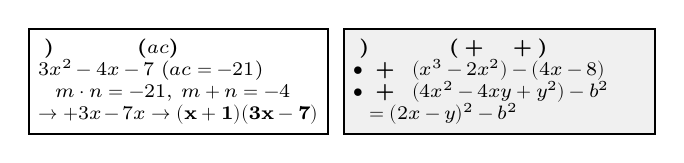
\begin{tikzpicture}[every node/.style={font=\scriptsize, text=black}]
  \node[draw=black, line width=0.9pt, fill=white, text width=3.55cm, align=left, inner sep=3.5pt] (split) at (0,0) {
    \textbf{១) បំបែកតួកណ្ដាល ($ac$)៖}\\
    $3x^2 - 4x - 7$ ($ac = -21$)\\
    រក $m\cdot n = -21,\; m+n = -4$\\
    $\to +3x - 7x \to \mathbf{(x+1)(3x-7)}$
  };
  \node[draw=black, line width=0.9pt, fill=gray!12, text width=3.70cm, align=left, inner sep=3.5pt, right=5pt of split] (grp) {
    \textbf{២) ផ្ដុំតួ ៤ តួ (២+២ ឬ ៣+១)៖}\\
    $\bullet$ \textbf{២+២៖} $(x^3-2x^2) - (4x-8)$\\
    $\bullet$ \textbf{៣+១៖} $(4x^2-4xy+y^2) - b^2$\\
    \hspace*{0.8em}$= (2x-y)^2 - b^2$
  };
\end{tikzpicture}}

\begin{document}
\fontsize{10pt}{15.2pt}\selectfont

% -------------------- ក្បាលកិច្ចតែងការ (Header) --------------------
\begin{center}
  {\muol\fontsize{11pt}{16pt}\selectfont ព្រះរាជាណាចក្រកម្ពុជា}\\[2pt]
  {\muol\fontsize{10pt}{15pt}\selectfont ជាតិ សាសនា ព្រះមហាក្សត្រ}\\[1pt]
  \khmflourish
\end{center}

\vspace{-28pt}
{\muol\fontsize{9.5pt}{12.5pt}\selectfont
មន្ទីរអប់រំ យុវជន និងកីឡា ខេត្តកំពង់ធំ\\
ការិយាល័យអប់រំ យុវជន និងកីឡា ស្រុកកំពង់ស្វាយ\\
អនុវិទ្យាល័យព្រះក្រសាំង}

\vspace{1pt}
\begin{center}
  {\muol\fontsize{10pt}{14pt}\selectfont កិច្ចតែងការបង្រៀន}
\end{center}
\vspace{0pt}

% -------------------- ព័ត៌មានទូទៅ (Metadata) --------------------
{\renewcommand{\arraystretch}{0.95}
\hspace*{4.05cm}%
\begin{tabular}{@{}l l l@{}}
  - \hspace{0.35cm} មុខវិជ្ជា & : & គណិតវិទ្យា ថ្នាក់ទី៨ \\
  - \hspace{0.35cm} ចំណងជើងមេរៀន & : & មេរៀនទី៥ កន្សោមពីជគណិត \\
  - \hspace{0.35cm} ចំណងជើងរង & : & ៤.២ (ត) របៀបផ្សេងៗក្នុងការដាក់កន្សោមជាផលគុណកត្តា \\
  - \hspace{0.35cm} រយៈពេល & : & ១ ម៉ោងសិក្សា (៥០ នាទី) \\
  - \hspace{0.35cm} បង្រៀនដោយ & : & ហុក ប៊ុនថែន \\
  - \hspace{0.35cm} កាលបរិច្ឆេទ & : & ថ្ងៃសៅរ៍ ៣កើត ខែមិគសិរ ព.ស.២៥៧០ (១២ ធ្នូ ២០២៦) \\
\end{tabular}
}

\vspace{1pt}

% -------------------- I. វត្ថុបំណង --------------------
\textbf{I.} {\muol វត្ថុបំណង}\\[1pt]
\hspace*{0.55cm}%
\begin{tabular}{@{}l l L{14.2cm}@{}}
  \wcirc \hspace{0.25cm} វិជ្ជាសម្បទា & : & សិស្សប្រាប់បានត្រឹមត្រូវនូវយុទ្ធសាស្ត្រដាក់កន្សោមជាផលគុណកត្តាតាមវិធីបំពេញការេឈានទៅ $A^2-B^2$ វិធីបំបែកតួកណ្ដាល ($ac$) និងវិធីផ្ដុំតួជាគូ (២+២) ឬផ្ដុំជាការេទ្វេធាដកការេ (៣+១) (ទំ.៧១--៧២) ។ \\
  \wcirc \hspace{0.25cm} បំណិនសម្បទា & : & សិស្សដាក់ត្រីធាដឺក្រេទី២ $ax^2+bx+c$ និងពហុធា ៤ តួជាផលគុណកត្តាដឺក្រេទី១ បានត្រឹមត្រូវដោយជ្រើសរើសវិធីបំពេញការេ បំបែកតួកណ្ដាល ឬផ្ដុំតួបានសមស្រប ។ \\
  \wcirc \hspace{0.25cm} ចរិយាសម្បទា & : & សិស្សមានភាពអត់ធ្មត់ ហ្មត់ចត់ក្នុងការប្ដូរសញ្ញាក្នុងវង់ក្រចកពេលផ្ដុំតួ និងចេះផ្ទៀងផ្ទាត់ចម្លើយដោយគុណពន្លាតបញ្ច្រាសវិញយ៉ាងសកម្ម ។ \\
\end{tabular}

\vspace{1pt}

% -------------------- II. សម្ភារៈឧបទេស --------------------
\textbf{II.} {\muol សម្ភារៈឧបទេស}\\[1pt]
\hspace*{0.55cm}$\bullet$ \hspace{0.35cm} សៀវភៅសិក្សាគោលគណិតវិទ្យាថ្នាក់ទី៨ (ទំ.៧១--៧៤) ក្ដារខៀន ដីស បន្ទាត់ និងសន្លឹកកិច្ចការសិស្សស-ខ្មៅ (\en{Worksheet\_ALG58} ចំនួន ២ ទំព័រ \en{A4} ដោយគ្មានស្លាយ \en{LCD}) ។

\vspace{1pt}

% -------------------- III. វិធីសាស្រ្តបង្រៀន --------------------
\textbf{III.} {\muol វិធីសាស្រ្តបង្រៀន}\\[1pt]
\hspace*{0.55cm}$\bullet$ \hspace{0.35cm} គោលវិធីសិស្សមជ្ឈមណ្ឌលតាមគំរូ \en{5Es} រួមបញ្ចូល \textbf{ការប្រៀបធៀបយុទ្ធសាស្ត្រដាក់ជាផលគុណកត្តា៖ បំពេញការេ ទល់នឹង បំបែកតួកណ្ដាល និងការផ្ដុំតួ} (\en{Contrasting Factoring Strategies}; \en{O'Connor \& Norton, 2016; Marpa, 2019}) ។

\vspace{2pt}

% -------------------- IV. ដំណើរការបង្រៀន --------------------
\textbf{IV.} {\muol ដំណើរការបង្រៀន}\\[-6pt]

{\renewcommand{\arraystretch}{1.15}
\begin{longtable}{|L{5.50cm}|L{7.90cm}|L{4.80cm}|}
\hline
\multicolumn{1}{|c|}{\cellcolor{headgray}\muol សកម្មភាពគ្រូ} &
\multicolumn{1}{c|}{\cellcolor{headgray}\muol ខ្លឹមសារមេរៀន} &
\multicolumn{1}{c|}{\cellcolor{headgray}\muol សកម្មភាពសិស្ស} \\[2pt]
\hline
\endfirsthead

\hline
\multicolumn{1}{|c|}{\cellcolor{headgray}\muol សកម្មភាពគ្រូ} &
\multicolumn{1}{c|}{\cellcolor{headgray}\muol ខ្លឹមសារមេរៀន} &
\multicolumn{1}{c|}{\cellcolor{headgray}\muol សកម្មភាពសិស្ស} \\[2pt]
\hline
\endhead

\hline
\endfoot

% ==================== ជំហានទី១ (2min) ====================
\stepheader{ជំហានទី១ ៖ រដ្ឋបាលថ្នាក់ (២ នាទី)}
$\bullet$ ពិនិត្យអវត្តមាន សណ្ដាប់ធ្នាប់ អនាម័យ និងសៀវភៅគោល \par\vspace{1pt}
$\bullet$ ចែកសន្លឹកកិច្ចការស-ខ្មៅ \en{Worksheet\_ALG58} ដល់សិស្សគ្រប់គ្នា
&
$\bullet$ វត្តមានសិស្ស ឯកសណ្ឋាន និងសណ្ដាប់ធ្នាប់ថ្នាក់រៀន \par
$\bullet$ សន្លឹកកិច្ចការសិស្ស \en{Worksheet\_ALG58} (ទំព័រ ១--២) លើតុរៀងៗខ្លួន
&
$\circ$ ប្រធានថ្នាក់រាយការណ៍អវត្តមាន \par
$\circ$ សរសេរឈ្មោះលើសន្លឹកកិច្ចការ \\
\hline

% ==================== ជំហានទី២ (9min) ====================
\stepheader{ជំហានទី២ ៖ កែកិច្ចការផ្ទះ រំលឹកមេរៀនចាស់ និងភ្ជាប់បញ្ហាថ្មី (៩ នាទី)}
\ditem \textbf{កែកិច្ចការផ្ទះ ($\le 3\unit{min}$)៖} \par
$\bullet$ ហៅសិស្ស ១ រូបឡើងកែលំហាត់ ១១ខ (ទំ.៧៣) និង ១៣ច (ទំ.៧៤) លើក្ដារខៀន
&
\textbf{កំណែកិច្ចការផ្ទះ (សៀវភៅគោល ទំ.៧៣--៧៤)៖} \par
១) $(3a^2 - 12a) - 5(a - 4) = 3a(a - 4) - 5(a - 4) = \mathbf{(a - 4)(3a - 5)}$ ។ \par
២) $5x^3 - 80x = 5x(x^2 - 16) = \mathbf{5x(x - 4)(x + 4)}$ ។
&
$\circ$ ផ្ទៀងផ្ទាត់ការចាប់កត្តារួមមុនប្រើផលដកពីរការេ \\[3pt]

\ditem \textbf{រំលឹកមេរៀនចាស់ ($3\unit{min}$)៖} \par
$\bullet$ សួររំលឹកពីការបំបែកផលដកពីរការេនៃកញ្ចប់ $(x - 1)^2 - 3^2$ និងកត្តារួមជាកញ្ចប់
&
\textbf{សំណួររំលឹកមូលដ្ឋានគ្រឹះ៖} \par
១) ផលដកពីរការេនៃកញ្ចប់៖ $(x - 1)^2 - 3^2 = (x - 1 - 3)(x - 1 + 3) = \mathbf{(x - 4)(x + 2)}$ ។ \par
២) ចាប់កញ្ចប់ទ្វេធា៖ $3x(x + 1) - 7(x + 1) = \mathbf{(x + 1)(3x - 7)}$ ។
&
$\circ$ គណនា $(x-1)^2 - 3^2$ និងចាប់កញ្ចប់ $(x+1)$ ជាកត្តារួម \\[3pt]

\fiveE{E1 - Engage} \timenote{(3 នាទី)} \par\vspace{1pt}
$\bullet$ សរសេរត្រីធា $A = x^2 - 2x - 8$ ប្រៀបធៀបនឹង $x^2 - 2x + 1$ លើក្ដារខៀន រួចឱ្យសិស្សទស្សន៍ទាយល្បិចបំប្លែងទៅជា $(x-1)^2 - 3^2$
&
\textbf{ស្ថានភាពភ្ជាប់បញ្ហា៖ ត្រីធាដែលមិនមែនជាការេទ្វេធា!} \par
ម្សិលមិញ $x^2 - 2x + 1 = (x-1)^2$ បំបែកបានភ្លាម ។ ចុះ $A = x^2 - 2x - 8$ (ទំ.៧១) គ្មានកត្តារួម ហើយ $-8$ ក៏មិនមែនជាការេដែរ! ប៉ុន្តែមិញនេះយើងឃើញ $(x-1)^2 - 3^2 = (x-4)(x+2) = x^2 - 2x - 8$! \par
\hspace*{0.3em}– \textbf{សំណួរបេសកកម្ម៖} «តើយើងអាចថែម-ថយចំនួនណាដើម្បីបំពេញ $x^2-2x$ ឱ្យក្លាយជាការេទ្វេធា? ចុះបើបំបែកតួកណ្ដាល $-2x$ វិញ ត្រូវបំបែកយ៉ាងដូចម្ដេច?»
&
$\circ$ សង្កេតទំនាក់ទំនង $x^2 - 2x + 1 - 1 - 8 = (x-1)^2 - 9$ \par
$\circ$ គូសធីកការទស្សន៍ទាយមុនរៀនក្នុងផ្នែកទី១ នៃសន្លឹកកិច្ចការ \\[3pt]

& \cfig{\figEngageALGEight} & \\
\hline

% ==================== ជំហានទី៣ (17min) ====================
\stepheader{ជំហានទី៣ ៖ មេរៀនថ្មី — បំពេញការេ បំបែកតួកណ្ដាល និងការផ្ដុំតួ (១៧ នាទី)}
\fiveE{E2 - Explore} \timenote{(11 នាទី)} \par\vspace{1pt}
\ditem \textbf{សកម្មភាពទី១៖ រុករកវិធីបំពេញការេឈានទៅ $A^2 - B^2$ ($5.5\unit{min}$)៖} \par
$\bullet$ ឱ្យសិស្សធ្វើការជាដៃគូលើ \textbf{ផ្នែកទី២ (ក)} នៃ \en{Worksheet\_ALG58} ដើម្បីបំពេញការេក្នុងឧទាហរណ៍ទី១ និងទី២ (ទំ.៧១)
&
\textbf{ការរុករកទី១ (វិធីបំពេញការេ ឧទាហរណ៍ទី១--២ ទំ.៧១)៖} \par
$\bullet$ ឧទាហរណ៍១៖ $A = x^2 - 2x - 8 = (x^2 - 2x + 1) - 1 - 8 = (x - 1)^2 - 3^2 = \mathbf{(x - 4)(x + 2)}$ ។ \par
$\bullet$ ឧទាហរណ៍២៖ $E = 9t^4 - 28t^2 + 16 = (9t^4 - 24t^2 + 16) + 24t^2 - 28t^2 = (3t^2 - 4)^2 - (2t)^2 = \mathbf{(3t^2 - 2t - 4)(3t^2 + 2t - 4)}$ ។ \par
\textit{(ប្រៀបធៀប៖ ចំពោះ $x^2-2x-8$ បើបំបែក $-2x = 2x - 4x$ ក៏បាន $(x+2)(x-4)$ ដូចគ្នា!)}
&
$\circ$ បូក-ដក $1$ ដើម្បីបង្កើត $(x-1)^2 - 9$ \par
$\circ$ បំពេញតួកណ្ដាល $-24t^2$ រួចប្រើផលដកពីរការេដោយប្រយ័ត្នសញ្ញា $-4$ \\[3pt]

\ditem \textbf{សកម្មភាពទី២៖ រុករកវិធីបំបែកតួកណ្ដាល និងការផ្ដុំតួ ($5.5\unit{min}$)៖} \par
$\bullet$ ឱ្យដៃគូបន្តបំពេញ \textbf{ផ្នែកទី២ (ខ)}៖ បំបែកតួកណ្ដាលក្នុងឧទាហរណ៍ទី៣ និងប្រៀបធៀបផ្ដុំតួ ២+២ ទល់នឹង ៣+១ (លំហាត់គំរូ $A, B$ ទំ.៧១--៧២)
&
\textbf{ការរុករកទី២ (បំបែកតួកណ្ដាល និងផ្ដុំតួ ទំ.៧១--៧២)៖} \par
$\bullet$ ឧទាហរណ៍៣៖ $F = 3x^2 - 4x - 7 = 3x^2 + 3x - 7x - 7 = 3x(x+1) - 7(x+1) = \mathbf{(x+1)(3x-7)}$ ។ \par
$\bullet$ ផ្ដុំ ២+២ ($A$)៖ $x^3 - 2x^2 - 4x + 8 = x^2(x-2) - 4(x-2) = (x-2)(x^2-4) = \mathbf{(x-2)(x-2)(x+2)}$ ។ \par
$\bullet$ ផ្ដុំ ៣+១ ($B$)៖ $4x^2 + y^2 - b^2 - 4xy = (4x^2 - 4xy + y^2) - b^2 = (2x-y)^2 - b^2 = \mathbf{(2x-y-b)(2x-y+b)}$ ។
&
$\circ$ រកពីរចំនួន $+3$ និង $-7$ ដែលគុណស្មើ $3(-7)=-21$ និងបូកស្មើ $-4$ \par
$\circ$ ប្រៀបធៀបពេលណាផ្ដុំ ២+២ និងពេលណាផ្ដុំ ៣+១ \\[3pt]

\fiveE{E3 - Explain} \timenote{(6 នាទី)} \par\vspace{1pt}
$\bullet$ ហៅតំណាងដៃគូឡើងសង្ខេបវិធីបំពេញការេ និងវិធីបំបែកតួកណ្ដាលលើក្ដារខៀន
&
\textbf{សង្ខេបខ្លឹមសារគោល៖ យុទ្ធសាស្ត្រទាំង ៤ សម្រាប់កន្សោមស្មុគស្មាញ (ទំ.៧១--៧២)} \par
$\bullet$ \cnum{1} \textbf{បំពេញការេ៖} បូក-ដក $\left(\frac{b}{2}\right)^2$ លើ $x^2+bx+c$ ឱ្យចេញទម្រង់ $A^2 - B^2 = (A-B)(A+B)$ ។ \par
$\bullet$ \cnum{2} \textbf{បំបែកតួកណ្ដាល ($ax^2+bx+c$)៖} រក $m, n$ ដែល $m\cdot n = ac$ និង $m + n = b$ រួចបំបែក $bx = mx + nx$ ។
&
$\circ$ ឡើងសរសេរលក្ខខណ្ឌ $m\cdot n = ac$ និង $m + n = b$ លើក្ដារខៀន \\[3pt]

$\bullet$ សង្ខេបវិធីផ្ដុំតួជាគូ (២+២) និងការផ្ដុំ ៣ តួជាការេទ្វេធាដកការេ (៣+១)
&
$\bullet$ \cnum{3} \textbf{ផ្ដុំតួជាគូ (២+២)៖} ផ្ដុំពីរតួម្ដងដើម្បីទាញកញ្ចប់ទ្វេធារួម $ax+ay+bx+by = (a+b)(x+y)$ ។ \par
$\bullet$ \cnum{4} \textbf{ផ្ដុំតួជាការេទ្វេធាដកការេ (៣+១)៖} ផ្ដុំ ៣ តួជា $(A\pm B)^2$ ដកនឹង $C^2$ រួចប្រើ $a^2-b^2$ ។ \par
$\bullet$ \cnum{5} \textbf{ប្រយ័ត្នសញ្ញាដក៖} ពេលទាញសញ្ញាដកនៅមុខវង់ក្រចក ត្រូវប្ដូរសញ្ញាតួខាងក្នុង៖ $-4x + 8 = \mathbf{-4(x - 2)}$!
&
$\circ$ កត់ត្រាយុទ្ធសាស្ត្រ \cnum{1}--\cnum{4} និងចំណាំសញ្ញាដកចូលក្នុងប្រអប់ផ្នែកទី៣ \\
\hline

% ==================== ជំហានទី៤ (20min) ====================
\stepheader{ជំហានទី៤ ៖ ពង្រីកចំណេះដឹង និងវាយតម្លៃលទ្ធផលសិក្សា (២០ នាទី)}
\fiveE{E4 - Elaborate} \timenote{(10 នាទី)} \par\vspace{1pt}
\ditem \textbf{លំហាត់គំរូ $C, D$ (ទំ.៧១--៧២) និងលំហាត់ទី១៦ ក--ខ (ទំ.៧៤, $5\unit{min}$)៖} \par
$\bullet$ ដឹកនាំសិស្សដោះស្រាយលំហាត់គំរូ $C, D$ និងលំហាត់ទី១៦ ក--ខ ក្នុង \textbf{ផ្នែកទី៤ (១)} នៃសន្លឹកកិច្ចការ
&
\textbf{លំហាត់គំរូ $C, D$ (ទំ.៧១--៧២) និងបំពេញការេ ១៦ ក--ខ (ទំ.៧៤)៖} \par
$\bullet$ $C = (a-4)(y+2) - (a-4)(3y+2) = (a-4)(y+2-3y-2) = \mathbf{-2y(a-4)}$ ។ \par
$\bullet$ $D = x^3(x+1) + y^3(x+1) = (x+1)(x^3+y^3) = \mathbf{(x+1)(x+y)(x^2-xy+y^2)}$ ។ \par
$\bullet$ លំហាត់ ១៦ ក--ខ៖ ចំពោះ $A = b^2 + 8b + 15$ ត្រូវថែម $\mathbf{16}$ លើ $b^2+8b$ ដើម្បីបាន $(b+4)^2$ $\implies A = (b+4)^2 - 16 + 15 = (b+4)^2 - 1^2 = \mathbf{(b+3)(b+5)}$ ។
&
$\circ$ ប្រុងប្រយ័ត្នការលុបវង់ក្រចក $-(3y+2) = -3y-2$ និងការបំបែក $x^3+y^3$ បន្តទៀត \\[3pt]

\ditem \textbf{អនុវត្តបំបែកតួកណ្ដាលលើត្រីធា $ax^2+bx+c$ (ទំ.៧៤, $5\unit{min}$)៖} \par
$\bullet$ ដឹកនាំសិស្សអនុវត្តវិធីបំបែកតួកណ្ដាលលើលំហាត់ទី១៥ (ក, ខ, ង ទំ.៧៤)
&
\textbf{ការដាក់ត្រីធាជាផលគុណកត្តាតាមបំបែកតួកណ្ដាល (ទំ.៧៤)៖} \par
$\bullet$ ១៥ក៖ $x^2 + 3x + 2 = x^2 + x + 2x + 2 = \mathbf{(x+1)(x+2)}$ ($1\times 2 = 2,\; 1+2 = 3$) ។ \par
$\bullet$ ១៥ខ៖ $3x^2 + 14x + 8 = 3x^2 + 12x + 2x + 8 = 3x(x+4) + 2(x+4) = \mathbf{(x+4)(3x+2)}$ ($ac = 24$) ។ \par
$\bullet$ ១៥ង៖ $14a^2 + 18a - 20 = 2(7a^2 + 9a - 10) = 2(7a^2 + 14a - 5a - 10) = \mathbf{2(a+2)(7a-5)}$ ។
&
$\circ$ ចាប់កត្តារួម $2$ ចេញជាមុនក្នុងលំហាត់ ១៥ង ដើម្បីឱ្យលេខតូចងាយរក $m, n$ \\[3pt]

& \cfig{\figStratALGEight} & \\[3pt]

\fiveE{E5 - Evaluate} \timenote{(10 នាទី)} \par\vspace{1pt}
\ditem \textbf{អនុវត្តសំយោគចុងមេរៀនទី៥ (ទំ.៧៤, $6.5\unit{min}$)៖} \par
$\bullet$ ឱ្យសិស្សធ្វើលំហាត់ត្រីធា (១៥ឃ, ជ និង ១៦គ ទំ.៧៤) ដោយខ្លួនឯងក្នុងផ្នែកទី៥ (១)
&
\textbf{ចម្លើយហ្វឹកហាត់សំយោគចុងមេរៀនទី៥ (សៀវភៅគោល ទំ.៧៤)៖} \par
១) \textbf{ត្រីធា (១៦គ និង ១៥ឃ, ជ)៖} ក) $B = x^2 + 4x + 3 = \mathbf{(x+1)(x+3)}$ \;;\; ខ) $C = 4x^2 - 8x + 3 = (2x-2)^2 - 1 = \mathbf{(2x-3)(2x-1)}$ \;;\; គ) $2x^2 + 15x + 7 = \mathbf{(2x+1)(x+7)}$ \;;\; ឃ) $6x^2 + 5x + 1 = \mathbf{(2x+1)(3x+1)}$ ។
&
$\circ$ ជ្រើសរើសវិធីបំពេញការេ ឬបំបែកតួកណ្ដាល រួចគុណផ្ទៀងផ្ទាត់ក្នុងចិត្ត \\[3pt]

$\bullet$ ឱ្យសិស្សបន្តធ្វើលំហាត់ផ្ដុំតួ (១២ក, ច, ឆ ទំ.៧៤) រួចប្ដូរសន្លឹកកិច្ចការផ្ទៀងជាដៃគូ
&
២) \textbf{ផ្ដុំតួ និងកញ្ចប់កត្តារួម (ទំ.៧៤)៖} \par
\hspace*{0.3em}– ក) $8ax - bx + 8ay - by = x(8a-b) + y(8a-b) = \mathbf{(8a-b)(x+y)}$ \;;\; ខ) $ax + ay - 2bx - 2by = \mathbf{(a-2b)(x+y)}$ \par
\hspace*{0.3em}– គ) $(2x-3)(5x-1) - (2x-3)(x+1) = \mathbf{2(2x-3)(2x-1)}$ \;;\; ឃ) $x^2 - 6x + 9 - y^2 = \mathbf{(x-3-y)(x-3+y)}$ ។
&
$\circ$ ប្ដូរសន្លឹកកិច្ចការផ្ទៀងផ្ទាត់ការទាញ $2$ ចេញពី $(4x-2)$ (\en{Pause-Review}) \\[3pt]

\ditem \textbf{បិទបេសកកម្ម E1 និងតេស្តរហ័ស \en{Exit Check} ($3.5\unit{min}$)៖} \par
$\bullet$ សួរបិទបេសកកម្ម E1 និងឱ្យសិស្សគូសរង្វង់ជម្រើស \en{A--D}
&
$\bullet$ \textbf{បិទបេសកកម្ម E1៖} ថែម-ថយ $1$ លើ $x^2-2x-8$ បាន $(x-1)^2 - 9 = (x-4)(x+2)$ ឬបំបែក $-2x = 2x - 4x$ ។ \par
$\bullet$ \textbf{Exit Check៖} តើត្រីធា $x^2 - 4x - 5$ ដាក់ជាផលគុណកត្តាស្មើនឹងជម្រើសណា? \par
\en{A.} $(x - 5)(x - 1)$ \quad \en{B.} $(x + 5)(x - 1)$ \quad \graybox{\enbf{C.} $(x - 5)(x + 1)$ \ding{51}} \quad \en{D.} $(x - 2)^2 - 5$
&
$\circ$ ផ្ទៀង $(-5)(+1) = -5$ និង $-5 + 1 = -4$ រួចគូសរង្វង់ជម្រើស \textbf{C} \\
\hline

% ==================== ជំហានទី៥ (<=2min) ====================
\stepheader{ជំហានទី៥ ៖ កិច្ចការផ្ទះ និងបណ្ដាំផ្ញើ ($\le$ ២ នាទី)}
$\bullet$ កត់ត្រាកិច្ចការផ្ទះលើក្ដារខៀន (មានបោះពុម្ពស្រាប់នៅផ្នែកទី៦ នៃសន្លឹកកិច្ចការទំព័រទី២) \par
$\bullet$ រំលឹកឱ្យចាប់កត្តារួម $2$ ចេញពី $2a - 2b + 10 = 2(a - b + 5)$ ក្នុងលំហាត់ ១១ច
&
\textbf{កិច្ចការផ្ទះបញ្ចប់មេរៀនទី៥ (សៀវភៅសិក្សាគោល ទំ.៧៣--៧៤)៖} \par
១. \textbf{លំហាត់ទី១១ ច (ទំ.៧៣)៖} ដាក់ជាផលគុណកត្តា $(2a - 2b + 10) + (a - b)(a - b + 5)$ ។ \par
២. \textbf{លំហាត់ទី១២ (ខ, គ, ង) ទំ.៧៤៖} ខ) $(7a-1)^2 - (7a-1)(3a+2)$ \;;\; គ) $(2x+3)^2 - (2x+3)(5x-7)$ \;;\; ង) $(y-8)(4y-1) + y^2 - 8y$ ។ \par
៣. \textbf{លំហាត់ទី១៥ ញ (ទំ.៧៤)៖} ដាក់ជាផលគុណកត្តា $14x^2 + 32x + 8$ ។
&
$\circ$ កត់ត្រាកិច្ចការផ្ទះ និងរៀបចំសន្លឹកកិច្ចការមេរៀនទី៥ ទាំង ៨ ម៉ោងទុកក្នុងសឺមី \\[3pt]

$\bullet$ ណែនាំឱ្យអានមេរៀនថ្មី (មេរៀនទី៦) ជាមុនសម្រាប់សប្ដាហ៍ក្រោយ
&
$\bullet$ \textbf{អានជាមុន៖} \textbf{មេរៀនទី៦ កន្សោមសនិទាន} — ចំណុចទី១ និងទី២ \textbf{សញ្ញាណ និងតម្លៃលេខនៃកន្សោមសនិទាន} (ទំព័រ ៧៥--៧៦) ។
&
$\circ$ ទទួលបណ្ដាំផ្ញើ និងជម្រាបលាគ្រូ \\

\end{longtable}
}

\vspace{6pt}

% -------------------- ហត្ថលេខា (Signature Block) --------------------
\begin{flushright}
\begin{minipage}{9.6cm}
\centering
ថ្ងៃសៅរ៍ ៣កើត ខែមិគសិរ ឆ្នាំមមី អដ្ឋស័ក ពុទ្ធសករាជ ២៥៧០\\[2pt]
ព្រះក្រសាំង, ថ្ងៃទី១២ ខែធ្នូ ឆ្នាំ២០២៦\\[4pt]
{\muol គ្រូបង្រៀន}\\[32pt]
\hfill{\muol ហុក ប៊ុនថែន}\hspace*{1.4cm}
\end{minipage}
\end{flushright}

\end{document}
